\chapter{Electrones en un potencial periódico. Teoría de bandas.} \label{Ch:07}

Para mejorar algunas de las predicciones del modelo del gas de electrones libres se introduce ahora la interacción de los electrones con la red cristalina a través de un potencial periódico. Se sigue despreciando, sin embargo, la posible interacción de los electrones entre sí.

\section{Teorema de Bloch}

\begin{figure}[h!] \centering
    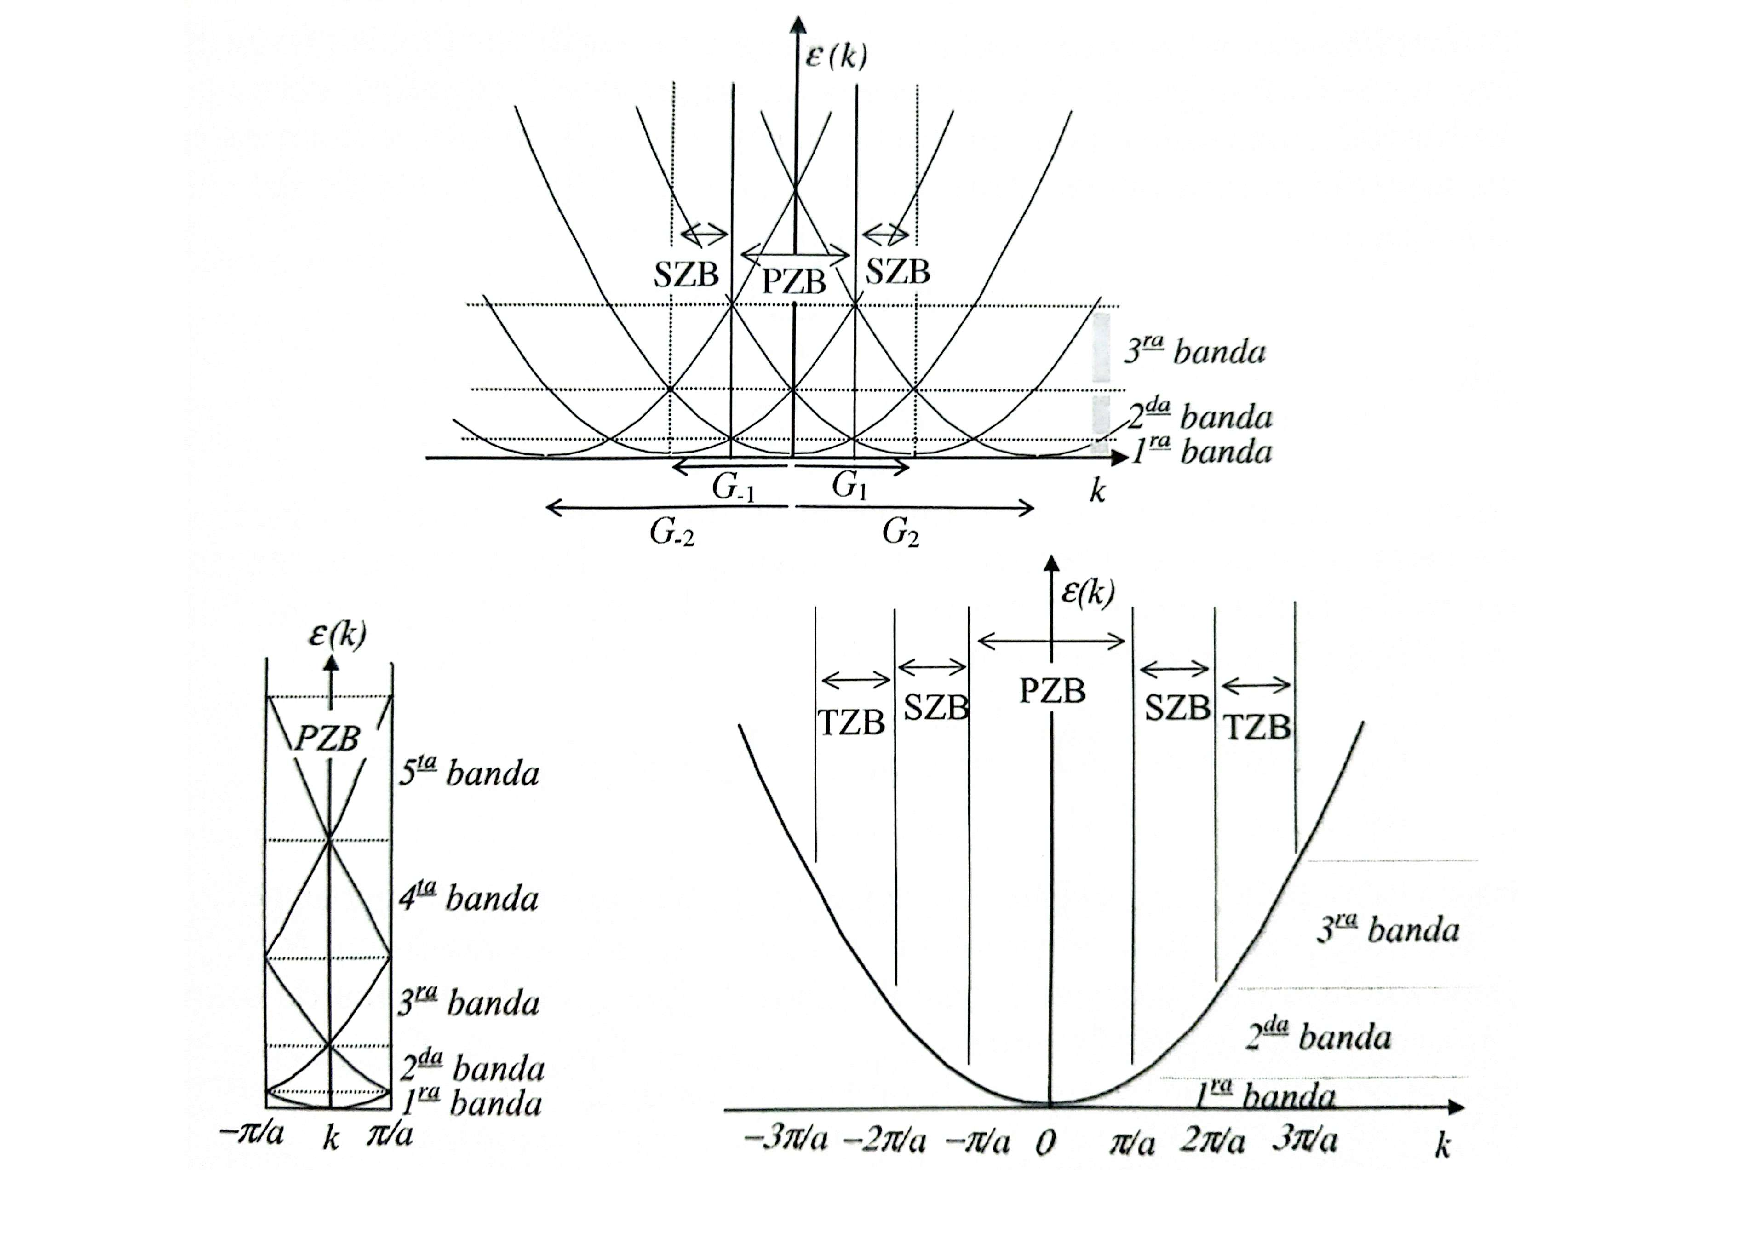
\includegraphics[scale=0.5]{Cuerpo/Ch_07/Fotos libro 1.pdf}
    \caption{Arriba: Esquema en zona periódica. Abajo: Esquemas en zona reducida (izquierda) y en zona extendida (derecha).}
    \label{Fig:07-01}
\end{figure}    


\section{Aproximación de red vacía}

\section{Ecuación de onda del electrón en un potencial periódico}

\section{Electrones cuasilibres}

\subsection{Gap de energía en los bordes de zona}
\begin{figure}[h!] \centering
    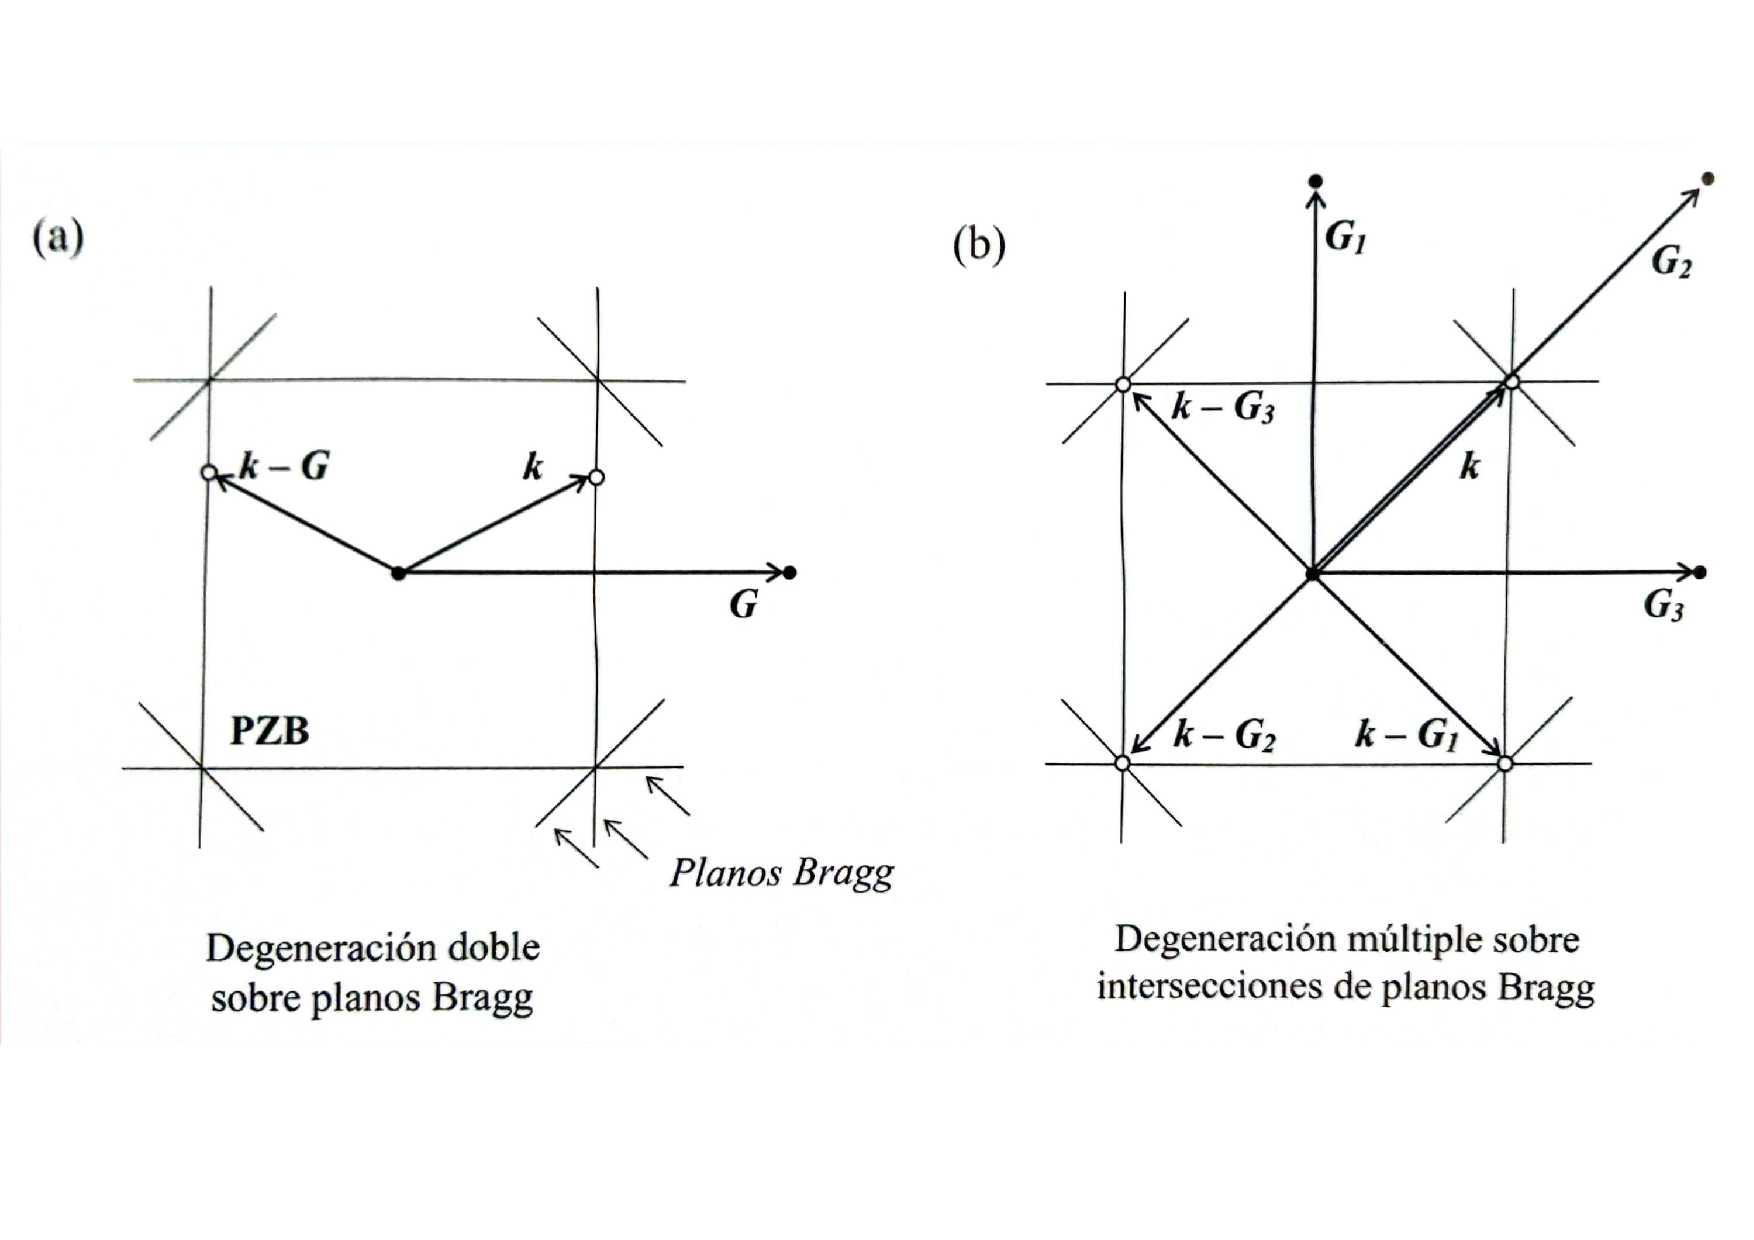
\includegraphics[scale=0.5]{Cuerpo/Ch_07/Fotos libro 2.pdf}
    \caption{(a) Ejemplo de estados doblemente degenerados sobre planos Bragg de una red cuadrada. (b) Estados cuádruplemente degenerados sobre las esquinas de la PZB de una red cuadrada.}
    \label{Fig:07-02}
\end{figure}    

\begin{figure}[h!] \centering
    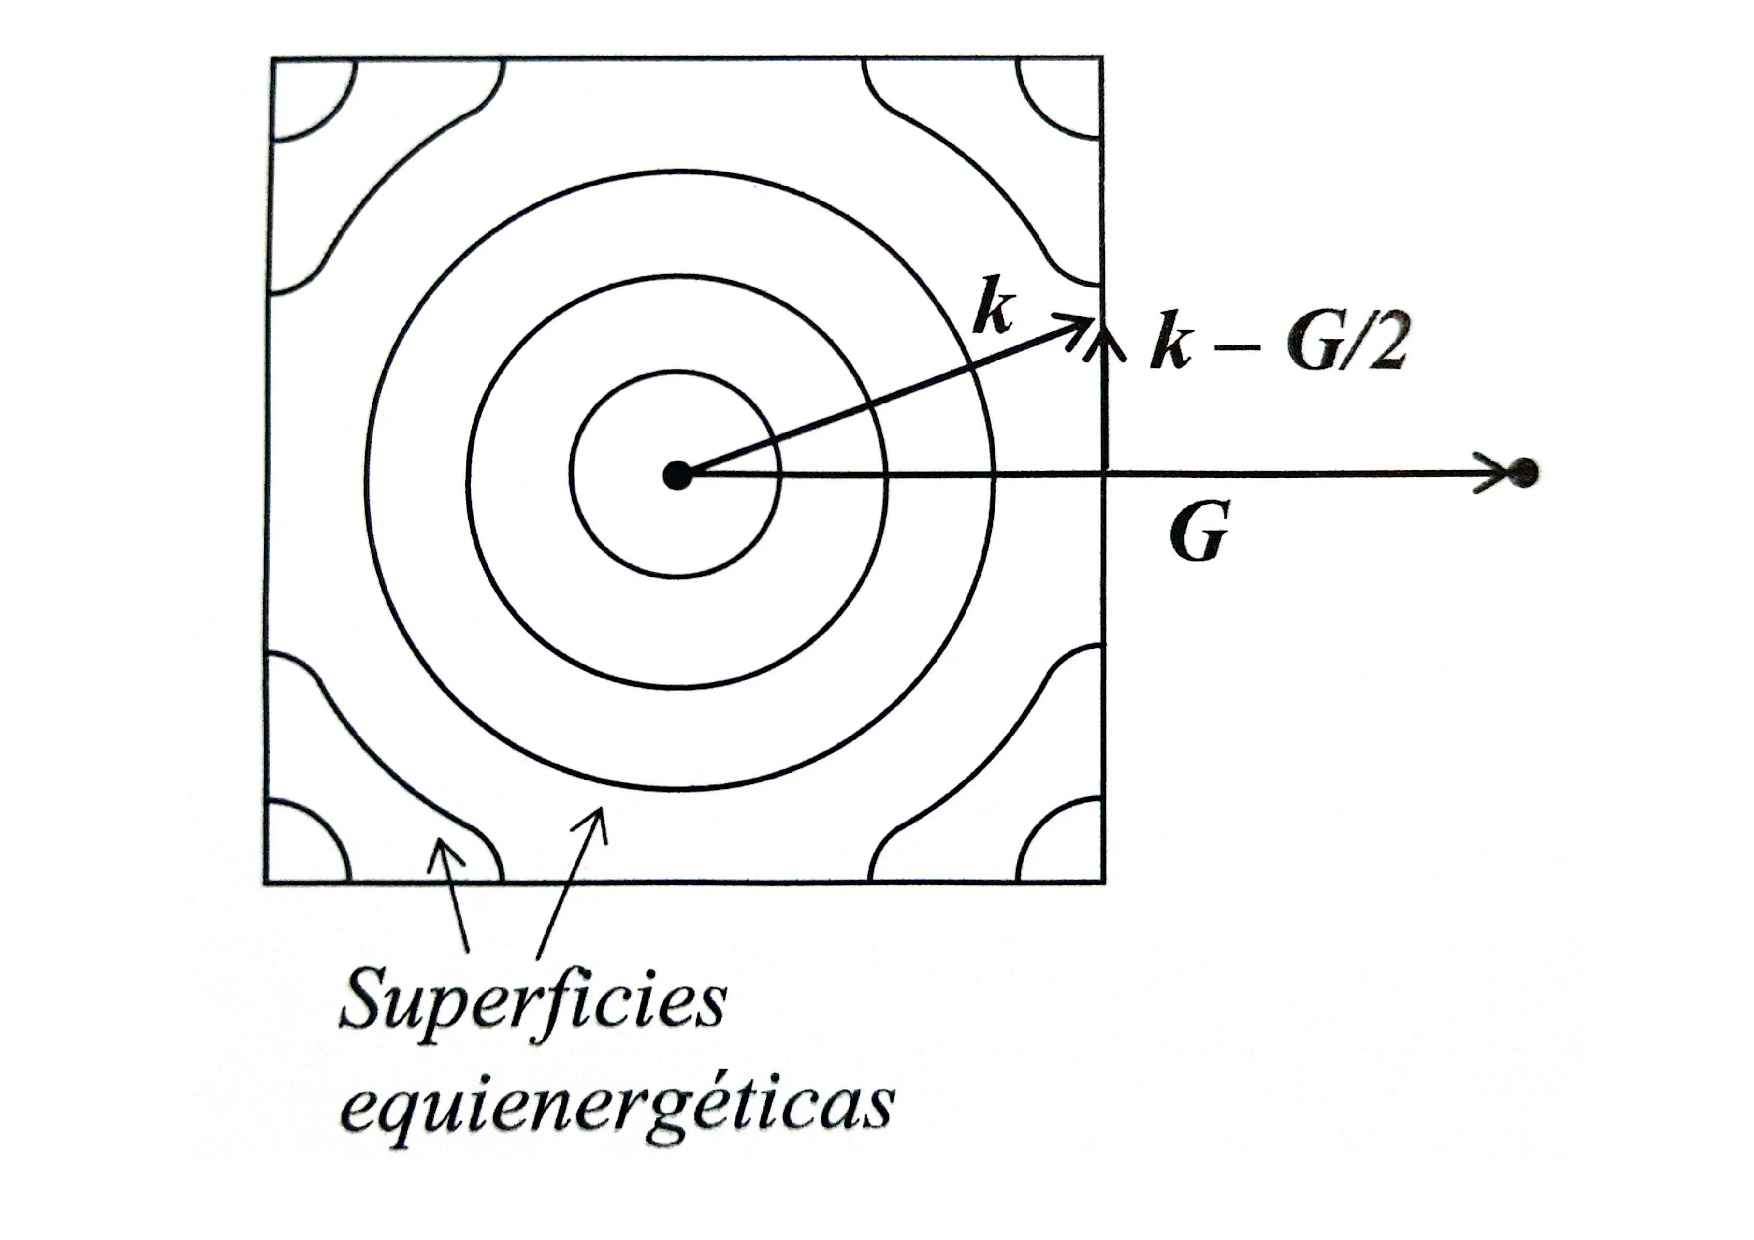
\includegraphics[scale=0.5]{Cuerpo/Ch_07/Fotos libro 3.pdf}
    \caption{Ejemplo de contornos equienergéticos en la PZB de una redcuadrada en la aproximación de electrones cuasilibres. Lejos de los planos de Bragg la aproximación de electrones libres es buena y los contornos son circulares. En los planos de Bragg, según se abre un gap de amplitud $2|U_{\Gn}|$. Según los contornos son perpendiculares a los planos de Bragg.}
    \label{Fig:07-03}
\end{figure}    

\begin{figure}[h!] \centering
    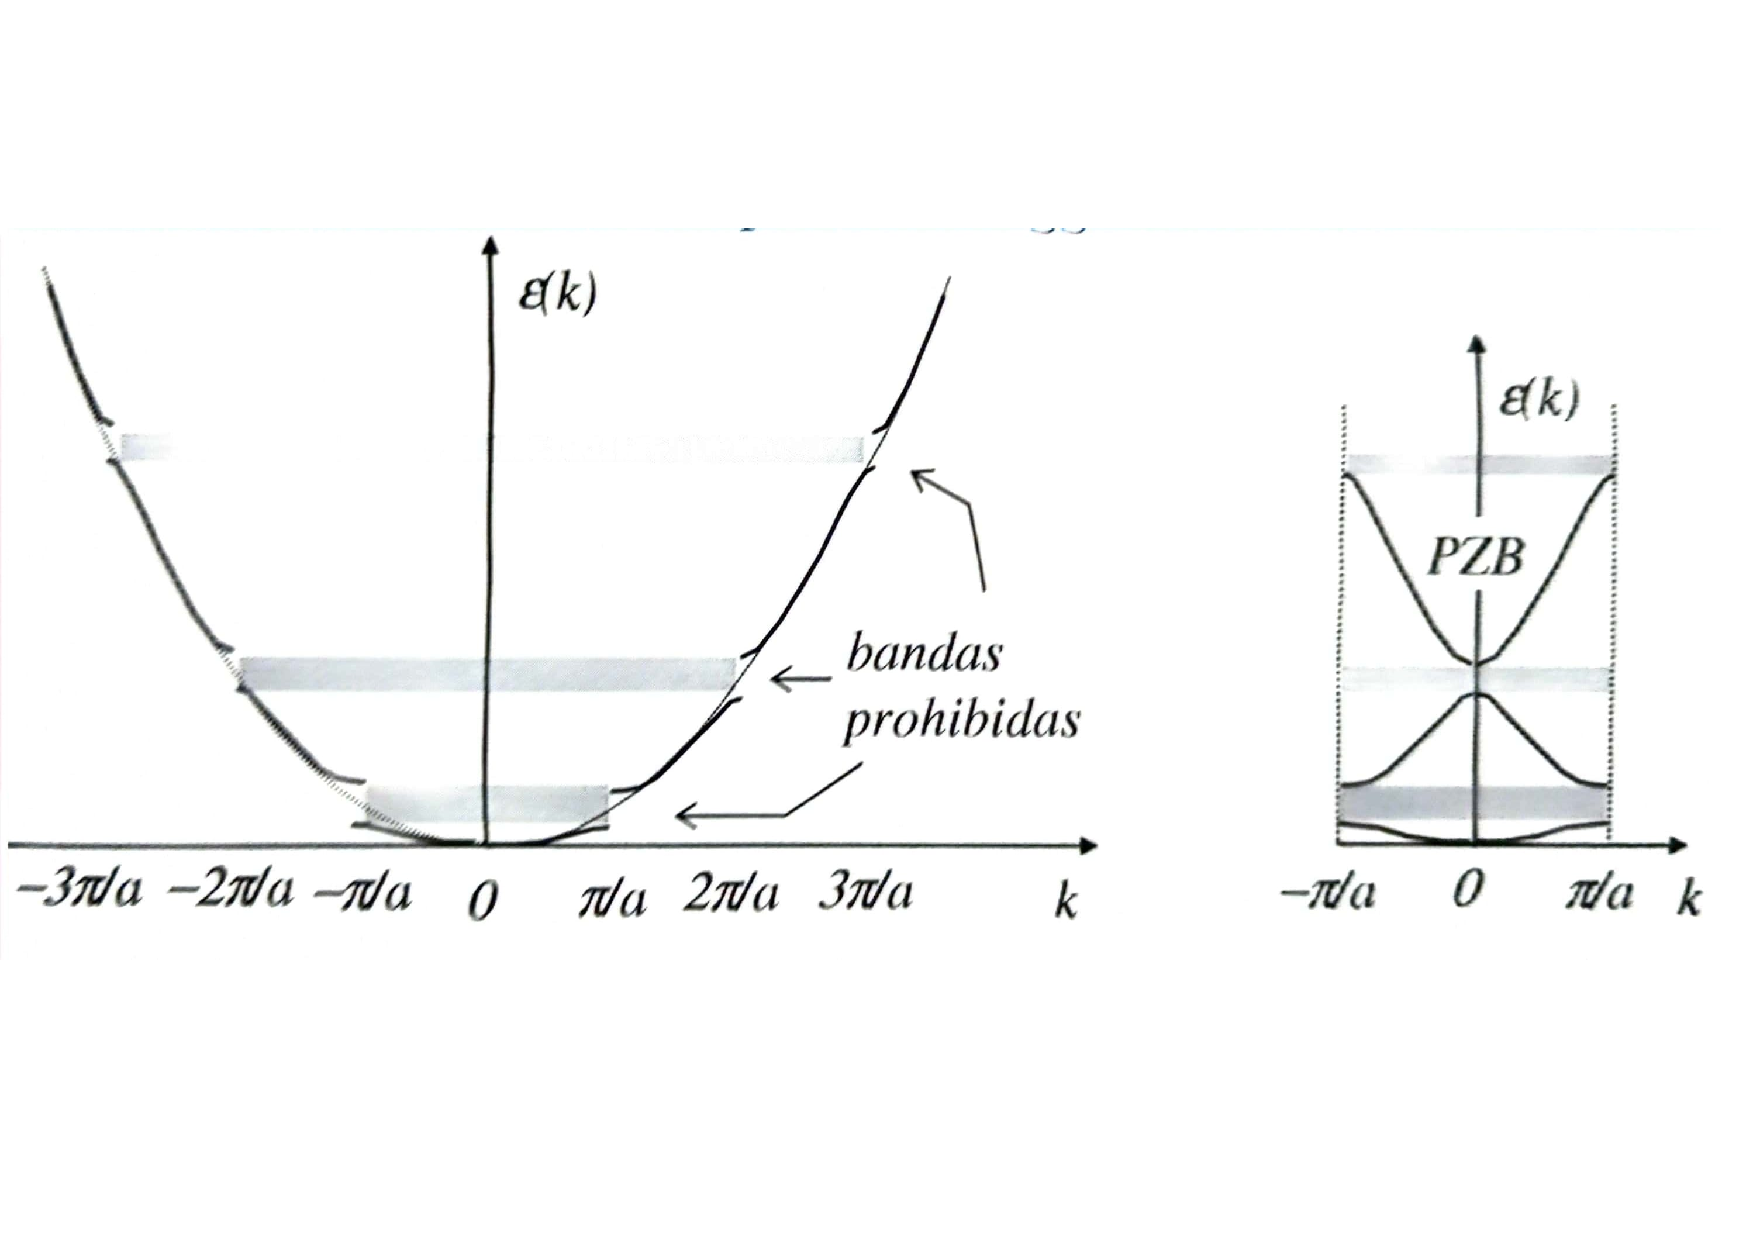
\includegraphics[scale=0.5]{Cuerpo/Ch_07/Fotos libro 4.pdf}
    \caption{Bandas prohibidas en los esquemas en zona extendida (izquierda) y reducida (derecha).}
    \label{Fig:07-04}
\end{figure}    

\section{Electrones fuertemente ligados}

\begin{figure}[h!] \centering
    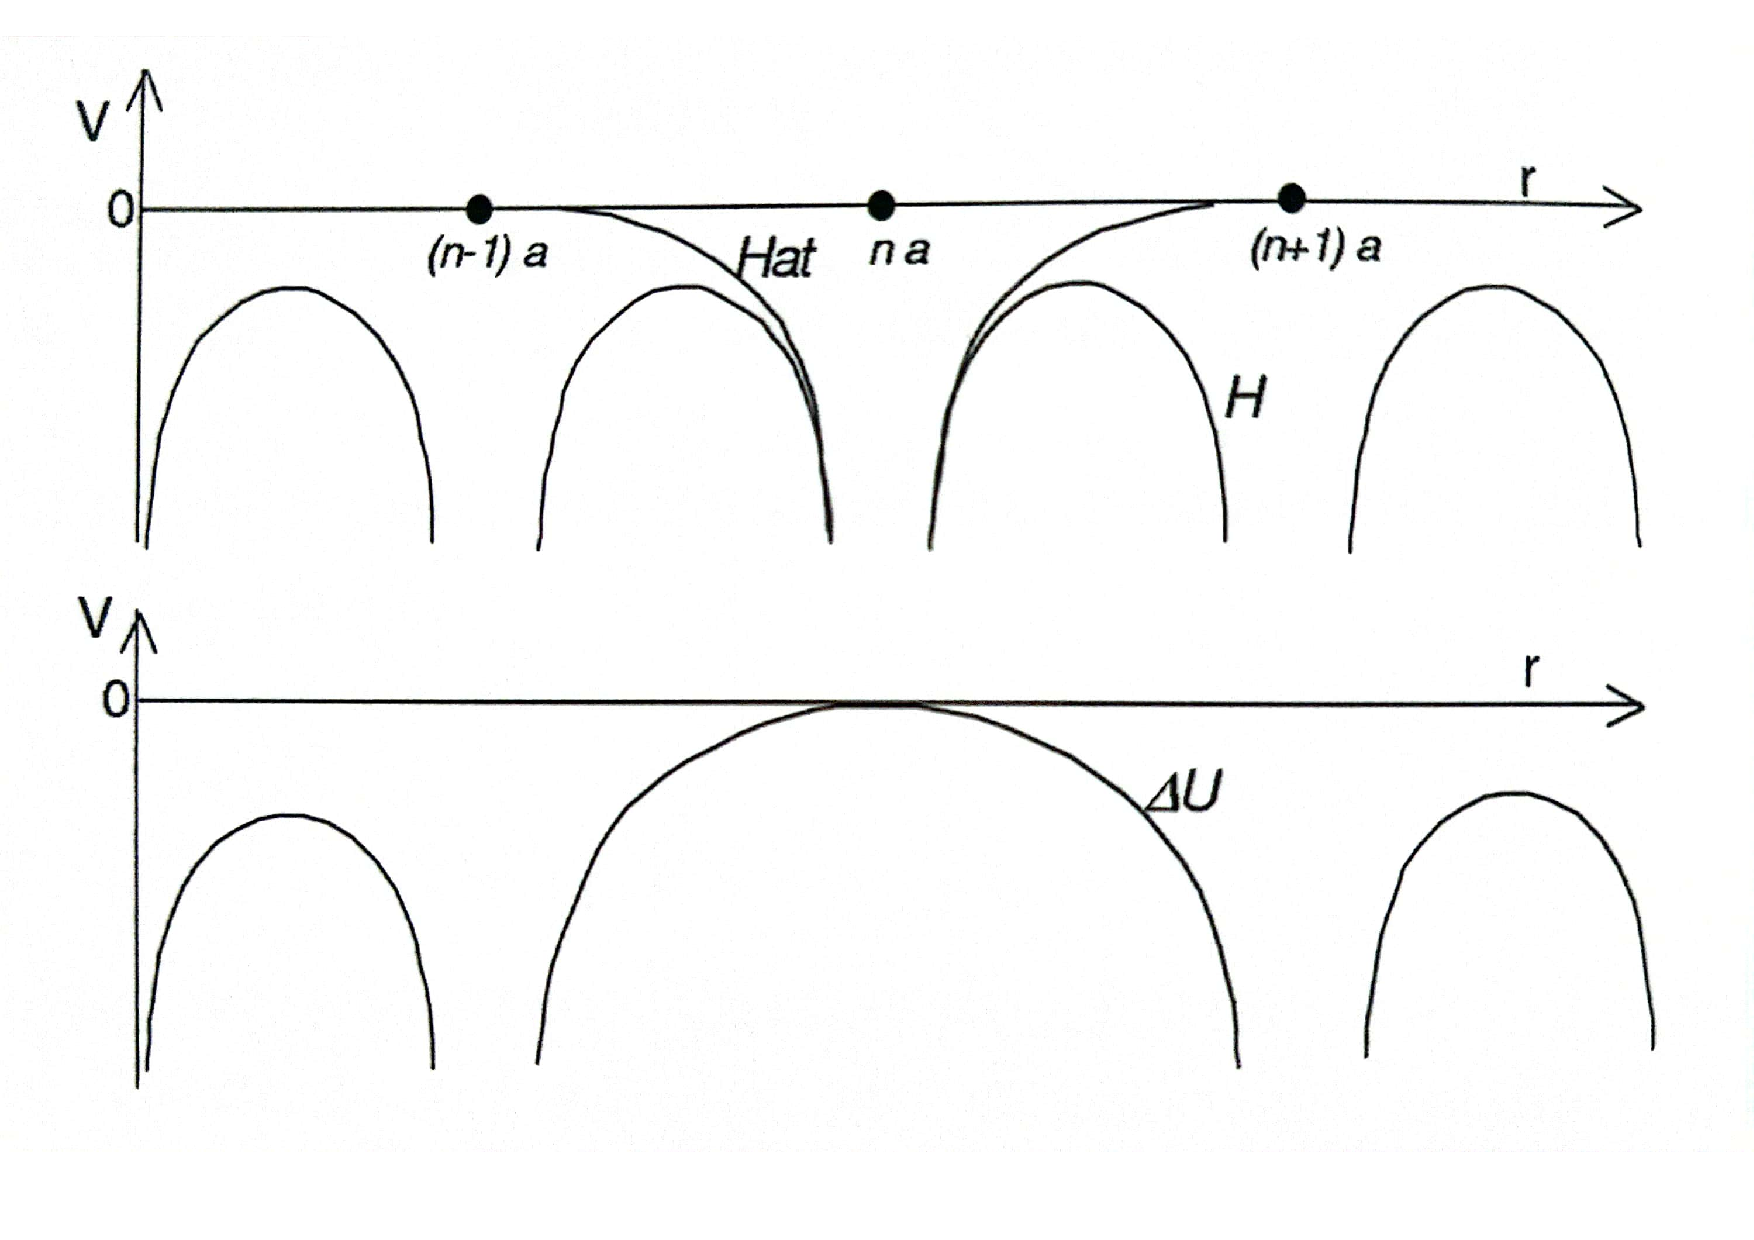
\includegraphics[scale=0.5]{Cuerpo/Ch_07/Fotos libro 5.pdf}
    \caption{Potencial periódico expresado como suma de un potencial atómico más una perturbación.}
    \label{Fig:07-05}
\end{figure}    
\begin{figure}[h!] \centering
    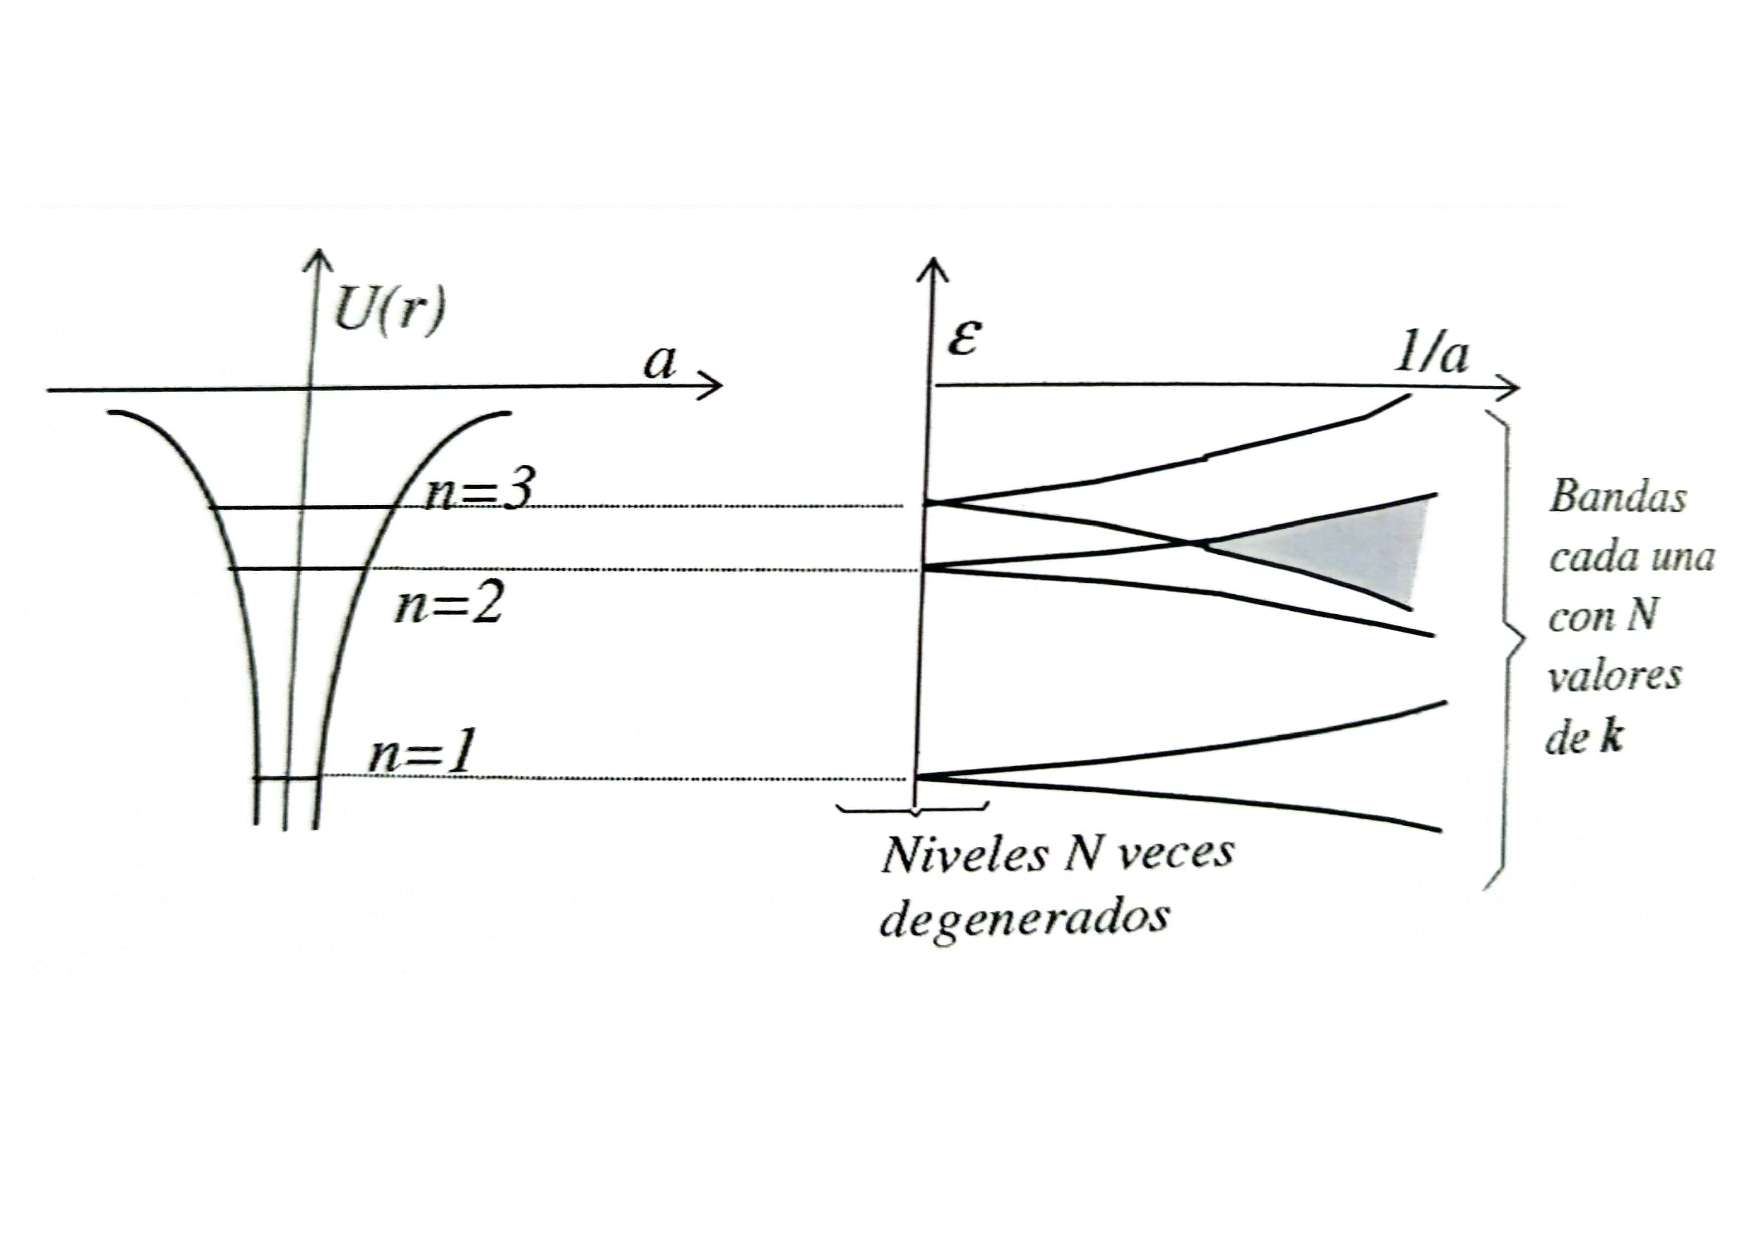
\includegraphics[scale=0.5]{Cuerpo/Ch_07/Fotos libro 6.pdf}
    \caption{Bandas de energía a partir de la aproximación de electrones fuertemente ligados. La zona sombreada representa el solapamiento entre la 1ª y 2ª bandas.}
    \label{Fig:07-06}
\end{figure}    

\section{Superficie de Fermi y zonas de Briollouin}
\begin{figure}[h!] \centering
    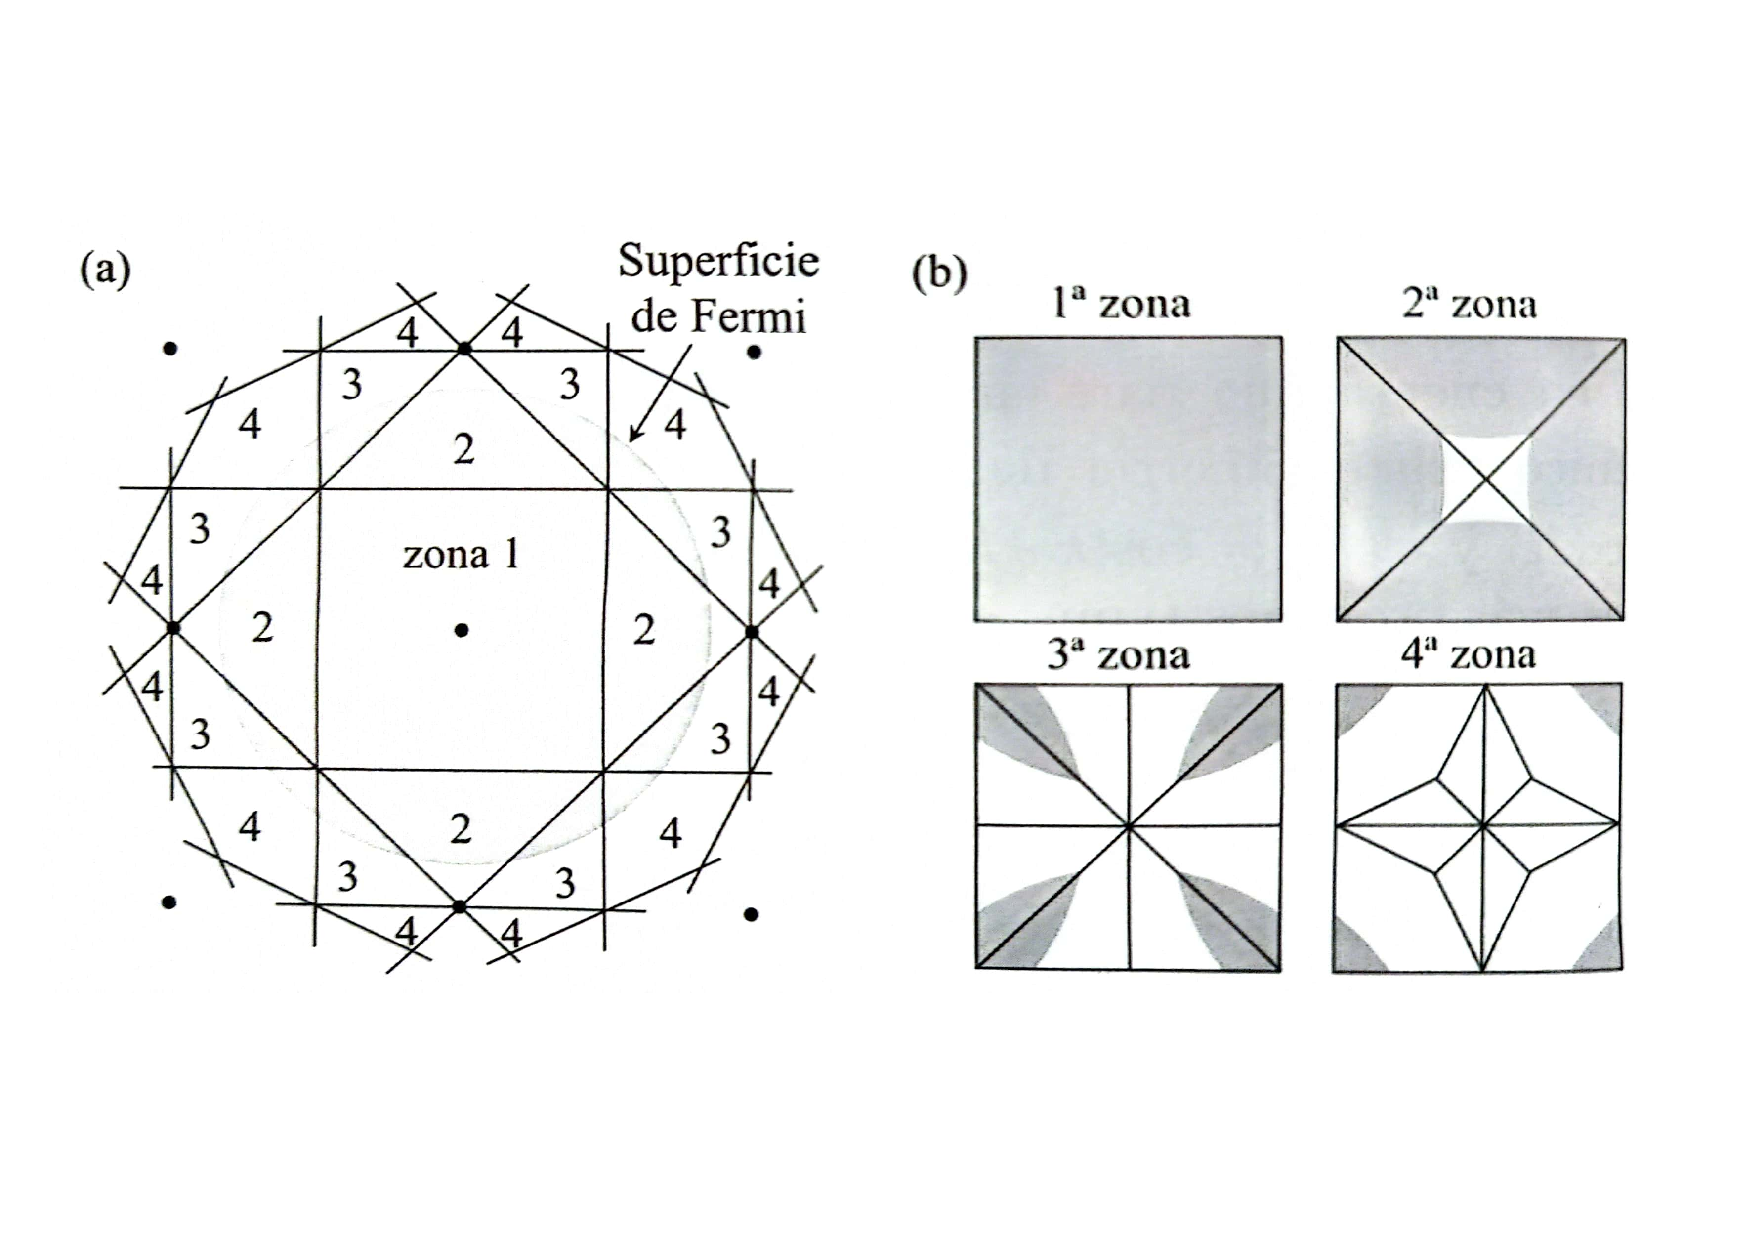
\includegraphics[scale=0.5]{Cuerpo/Ch_07/Fotos libro 7.pdf}
    \caption{1ª, 2ª, 3ª y 4ª zonas de Brillouin para una red cuadrada 2D, según los esquemas en zona extendida (a) y reducida (b). En gris se representan los estados ocupados.}
    \label{Fig:07-07}
\end{figure}    
\begin{figure}[h!] \centering
    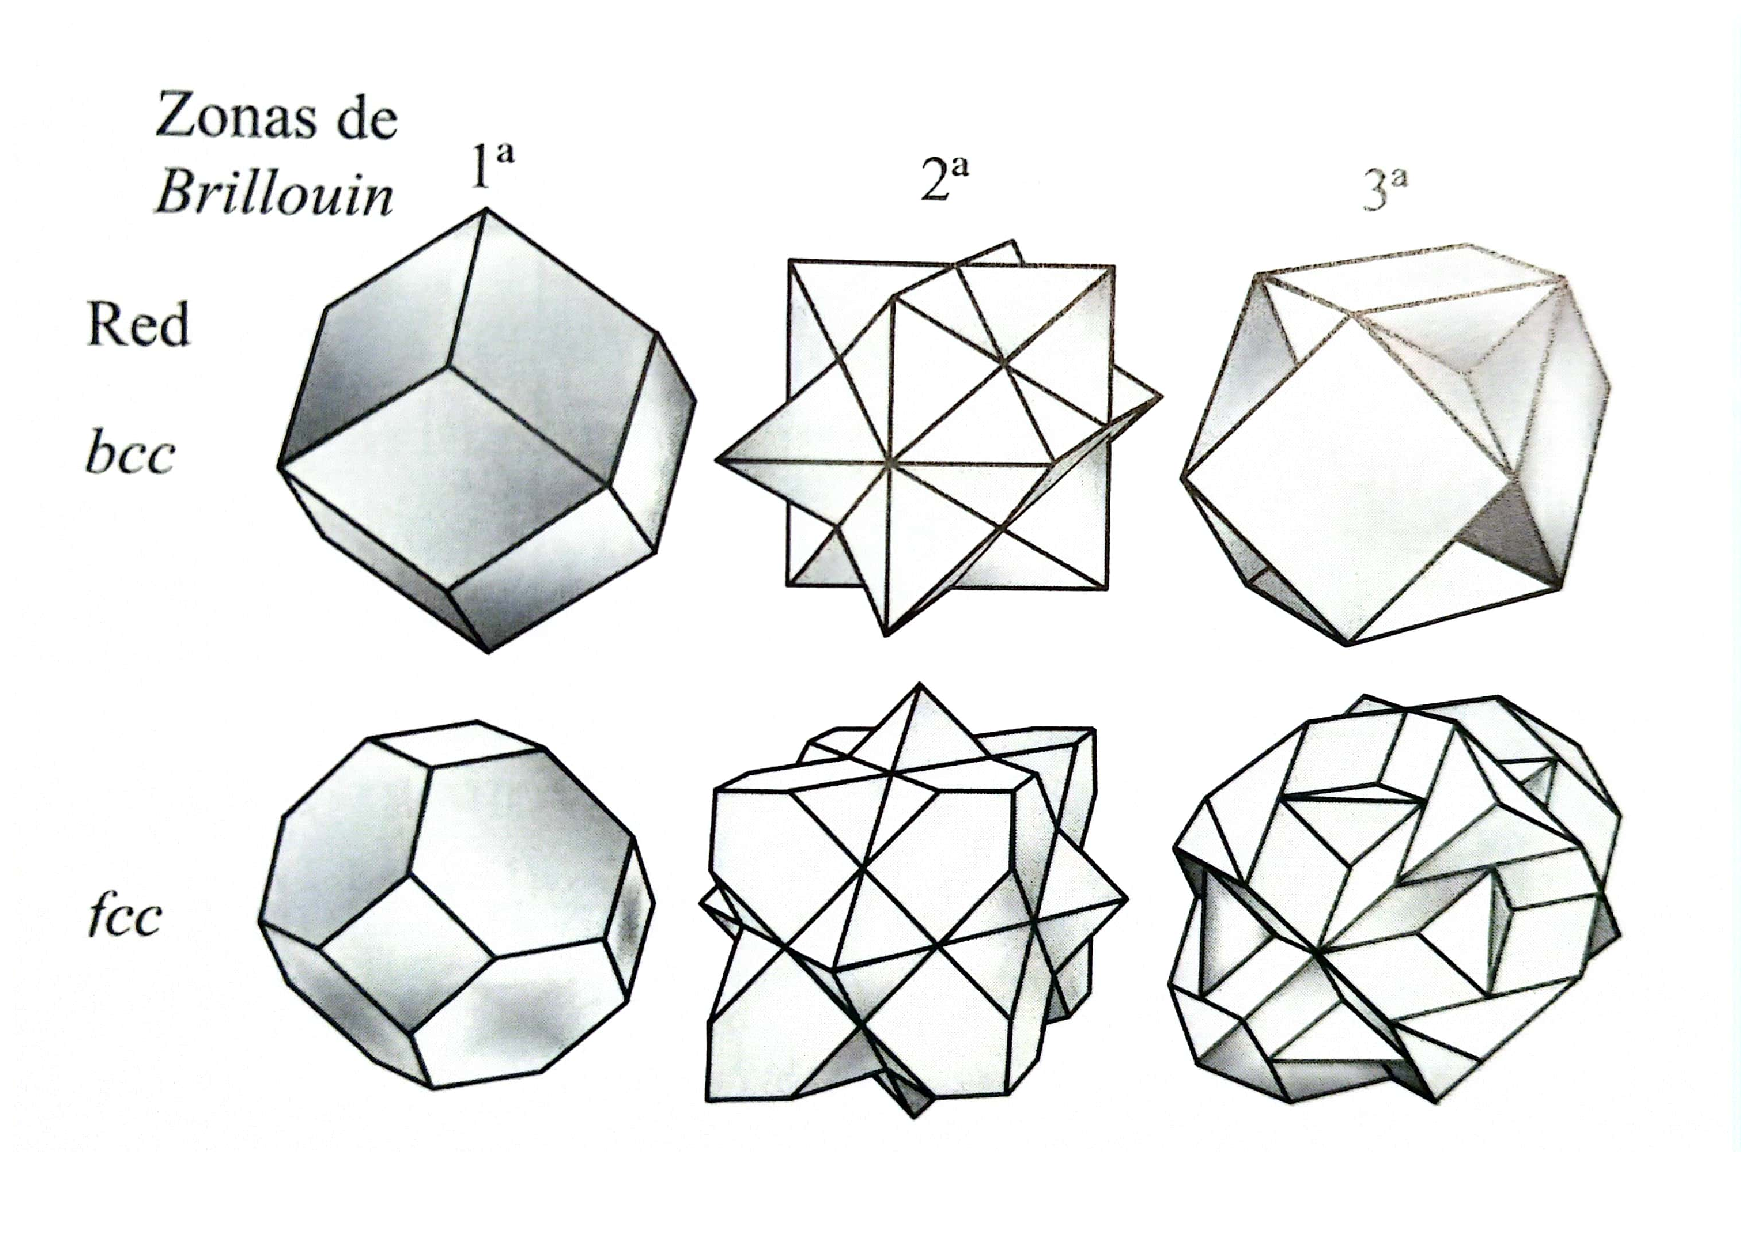
\includegraphics[scale=0.5]{Cuerpo/Ch_07/Fotos libro 8.pdf}
    \caption{Primeras zonas de Brillouin para las estructuras \bcc y \fcc, según el esquema en zona reducida.}
    \label{Fig:07-08}
\end{figure}    
\begin{figure}[h!] \centering
    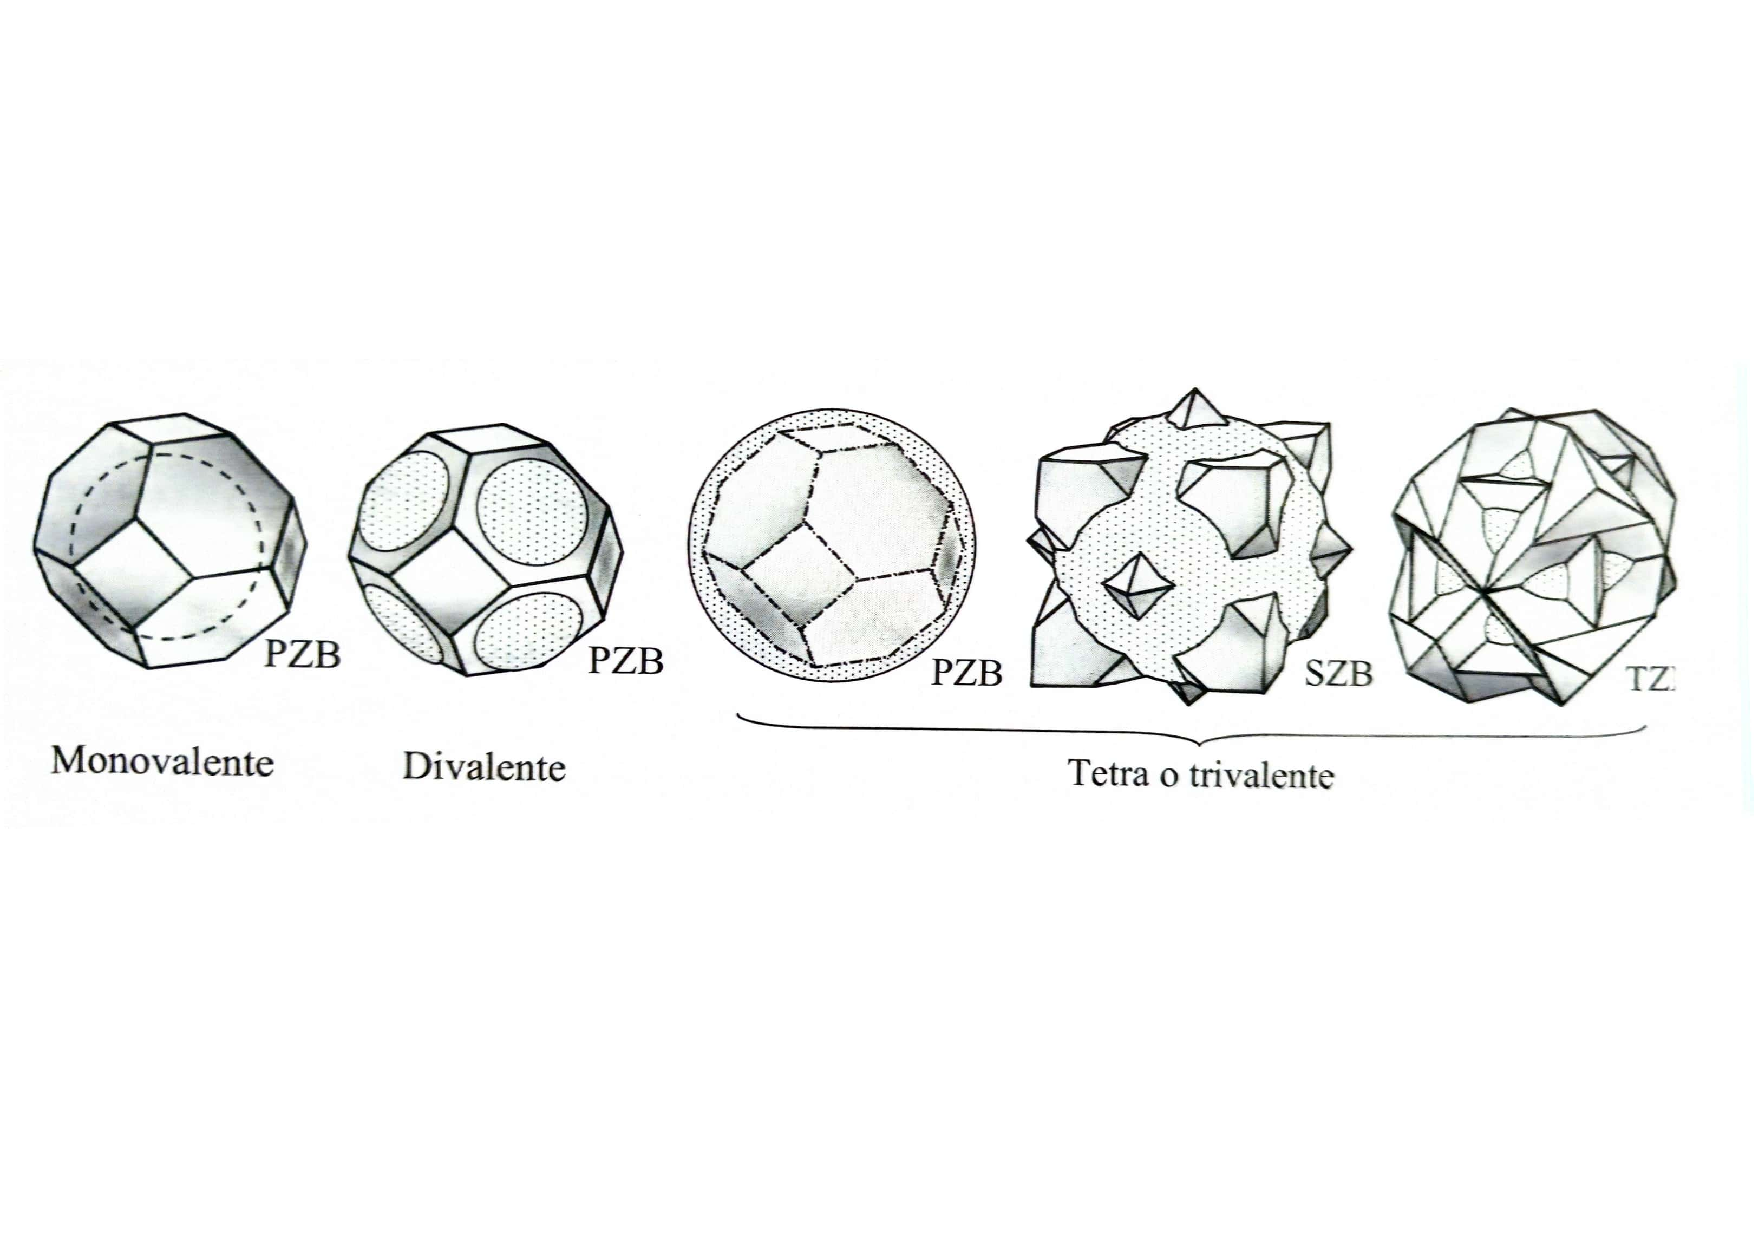
\includegraphics[scale=0.5]{Cuerpo/Ch_07/Fotos libro 9.pdf}
    \caption{Relación entre las primeras zonas de Brillouin de la estructura \fcc y la superficie de Fermi de electrones libres (esférica), según la valencia atómica.}
    \label{Fig:07-09}
\end{figure}    


\section{Metales, aislantes y semiconductores}
\begin{figure}[h!] \centering
    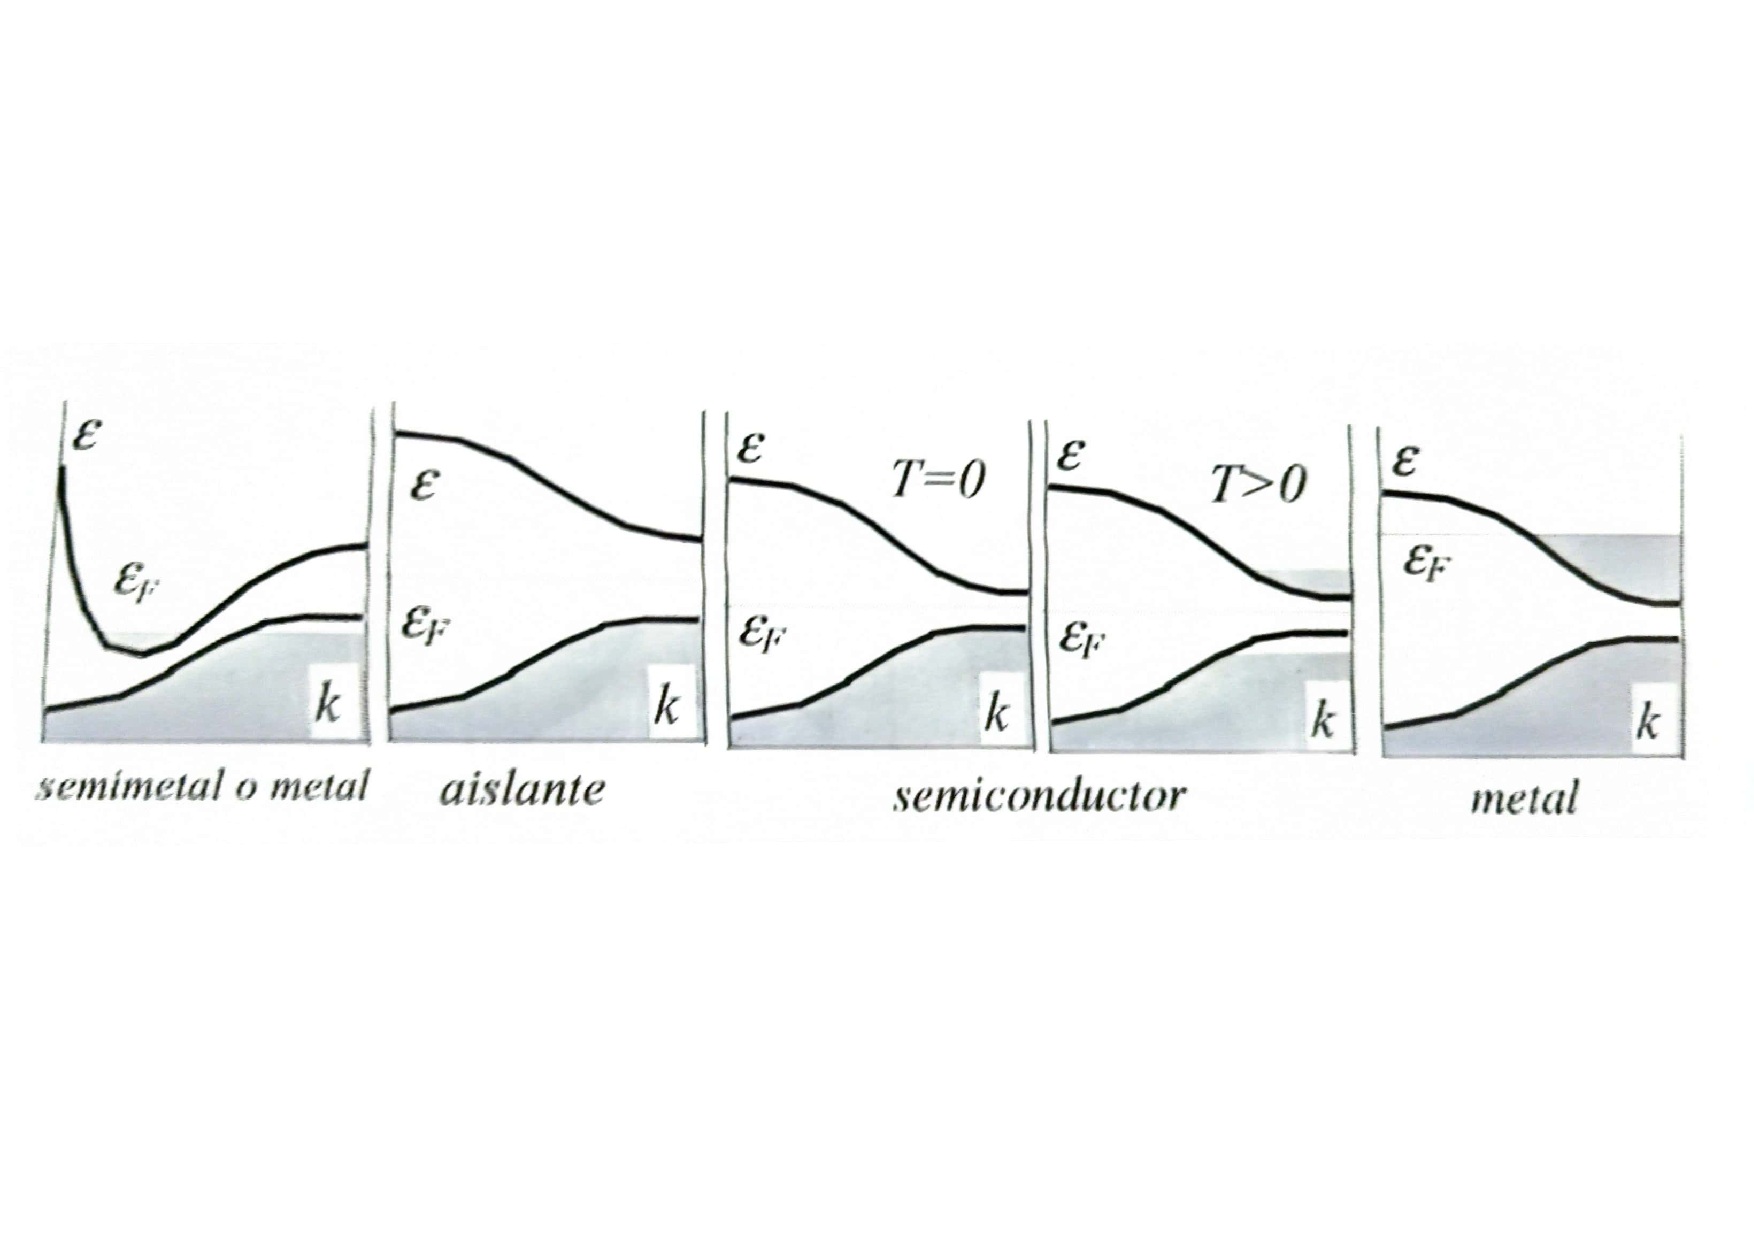
\includegraphics[scale=0.5]{Cuerpo/Ch_07/Fotos libro 10.pdf}
    \caption{Clasifiación de los sólidos según la relación que hay entre el nivel de Fermi y la estructura de bandas.}
    \label{Fig:07-10}
\end{figure}    
